%
%	WISS 2021サンプルファイル
%
%	2010/07/12 Ver 1.0 秋田 純一
%	2010/08/04 Ver 1.1 後藤 真孝
% 	2011/09/27  Ver 1.4 渡邊 恵太 (協力:五十嵐悠紀)
% 	2015/02/08  Ver 1.5 大槻 麻衣
% 	2015/07/09  Ver 1.6 大槻 麻衣(協力:三浦元喜)
% 	2016/05/26  Ver 1.7 大槻 麻衣
% 	2017/02/04  Ver 1.8 大槻 麻衣
%	2018/05/01  Ver 1.9 中村 裕美
%	2019/04/05  Ver 2.0 中村 裕美, 池松 香
%   2020/08/25  Ver 2.1 池松 香
%   2021/07/14  Ver 2.2 池松 香

\documentclass[twoside]{wiss}

\usepackage{ascmac}
\usepackage[dvips]{graphicx}
\usepackage{nidanfloat} %% appended in WISS2010 for Future Vision (2010/7/7:akita)
\usepackage{multicol}
%\usepackage{color,array}
%\usepackage{boxedminipage}

%% balance.styを追加 (2012/9/27:watanabe, Igarashi)
\usepackage{balance}    %% 最後のページの高さを揃えるために追加  (2012/9/27:watanabe, Igarashi)
%%% 最後のページの2段組の高さを揃える.\balanceを入れる.
%%% そろえたくないときは,\nobalance

%% urlのOverflow対策
\usepackage{url}

\journalhead{アプリ開発における異なる実践共同体の可視化システムの開発} %%%%%% ←← 著者において必ず記入すること

\begin{document}

\title{アプリ開発における異なる実践共同体の可視化システムの開発}
\etitle{}%2012年では英文タイトルは廃止されました.記入しないでください.
%
%注意
%
%
% WISS2016からシングルブラインドとなりました.投稿時に氏名と所属を記入してください.
\author{遠藤 勝也\affil{株式会社スタジオ・アルカナ}  武富 拓也\affil{明星大学}
  尼岡 利崇${}^\dag$}

\begin{abstract}
本研究では,アプリ開発における異なる実践共同体の参加の過程を
可視化するシステムを開発した.
% 著者らは過去に質的アプローチの観点から実践共同体の概念を用いて,
% 異なる背景を持つプロジェクトメンバの関係のあり方が,
% 開発されるアプリケーションにどのような影響を及ぼすかという研究を行った.
% その研究結果をもとにCSCW(Computer Supported Cooperative Work)の観点から,
% アプリケーション開発の過程における,
% 背景の異なるプロジェクトメンバの関わり方を可視化するシステムの開発を行った.
本システムを使用することにより,
異なる背景を持つメンバが参加するアプリ開発チームにおいて,
アプリの設計から実装をメンバ間の関係構築のあり方そのものからデザインすることの
支援を目的としている.
\end{abstract}

\maketitle

\section{はじめに}
\label{introduction}

現在のアプリ開発は,プログラマのみで完結することは少なく,
多様な背景を持つメンバと協働で行われる.またアプリ開発において,
TrelloやSlackといったICTツールが導入されている.
しかし異なる背景を有するコミュニティのメンバ同士がコミュニケーションを行う場合,
認識論の違いから主張の食い違いや対立が起きることもあるため\cite{conflict},
ICTツールを導入するだけでは異なる背景を持つメンバと協働でアプリ開発を行うには不十分であり,
メンバ間の人間関係がどのように作られていくかといったプロセスも見ていく必要があると考えられる.
そこで実践共同体\cite{Matsumoto}の布置という概念からメンバ間の関係性を捉えることが有効であると考えられる.
布置とは成員は単一の実践共同体のみに参加するものではなく,
複数の実践共同体に参加することを踏まえて,
複数の実践共同体における成員の振る舞いを捉える概念\ref{overlap}である.


そこで,著者らは実践共同体という概念を用いて,異なる背景を持つプロジェクトメンバが協働でタスクを行うことを支援する手法を提案する.実践共同体に布置という概念がある.
まず,過去に行った異なる背景を持つプロジェクトメンバの関係構築のあり方が,
開発されるアプリのデザインにどのような影響を及ぼすかという
研究の結果を見直し,課題を明らかにする.
そして明らかになった課題を解決するため,Trello APIからのデータを元にメンバ間の
関係を可視化することにより協働的に作業を促すシステムの提案を行った.

\begin{figure}[h]
    \centering
    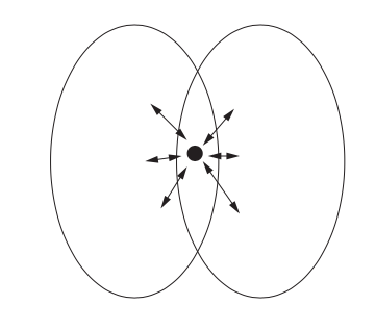
\includegraphics[width=0.5\textwidth]{img/overlap.eps}
    \caption{異なる実践共同体の協働のイメージ図}
    \label{overlap}
  \end{figure}

\section{先行研究}
\label{preResearch}
\subsection{学部横断型PBLのアプリ開発の過去研究について}

本研究は,過去に行った異なる背景を持つプロジェクトメンバの
関係構築のあり方が開発されるアプリのデザインにどのような影響を
及ぼすかという研究\cite{preStudy}の結果に基に行われたものである.
筆者らのこれまでの研究は大学の情報学部と人文学部の学部横断型PBL(Project based learning) を
対象として行われた.
研究結果では,プロジェクトメンバの関係構築の在り方が分業的関係か協働的関係に応じて、
プロジェクトメンバが所有する知識や技術といったリソースが
その人間関係のあり方に相応して開発プロセスに影響し,
アプリの機能やUIに現れるという示唆を得た.

専門性に関わるタスクしか関心を向けないという分業的な関係のあり方でアプリ開発を進めた際,
タスクをこなす際に,部分最適化する傾向があり制作された成果物は,
異なる実践共同体の専門を組み合せるにとどまっていた.
また異なる実践に価値をもつ両学科の学生が積極的にプロジェクトに参加する時期に齟齬がおきる傾向がみられた.

他方,自分の専門を超えて一緒に作業を行う時間を設ける協働的な関係のあり方
でアプリ開発を進めた際には,
短期的には非効率的に見えても,アプリ開発の過程に異なる実践共同体の実践,
つまりプログラムを書いている最中の意味の交渉や目的の修正や共有が行われ,
お互いの専門性を融合して成果物を作成することを可能にした.

\subsection{チームメンバの可視化手法について}

% チームメンバーをマネジメントする観点から,
% 可視化手法を用いた研究は多く存在する.
% Amrら\cite{Emotimonitor}は
% Trelloのカードに絵文字という感情表現の機能を
% 拡張することによりあるチームメンバの内面を可視化し
% プロジェクトの管理を支援している.
% 本研究ではTrello APIを用いて,プロジェクトに参加する
% チームメンバ間の関係性から
% プロジェクトの実践を支援することを目的としている. 

YUBOら\cite{D3jsOfCop}の研究では実践共同体の概念を用いて,
UXデザインという共通した目的を持つ実践共同体のメンバのやり取りを可視化している.
本研究では共通の目的を共有している実践共同体のみを分析するのではなく,
異なる目的をもつ複数の実践共同体のやり取りを含めて分析し可視化することに特徴がある.


\section{実践共同体の可視化システムについて}
\label{system}
% 3章にて
% 本研究が開発したシステムは,アプリ開発支援システムとして,
% 異分野横断的なアプリ開発において,
% 異なる実践共同体が協働的な関係構築を行うことで,
% お互いの実践を融合させてアプリ開発を支援することを目的としたシステムである.
% 使用場面として,ソフトウェアの開発手法の一つである
% アジャイル開発に活用されることを想定している.
% アジャイル開発とは機能単位の小さなサイクルで,
% 設計・開発・テストの工程を繰り返すことにより,
% 様々な状況の変化に対応しながら開発を進めていく手法である.
% 状況の変化に対応するため,
% 日毎にdaily scrumと呼ばれる短い時間での進捗の共有と反省を行う
% 打ち合わせの時間が設けられている.
% 開発したシステムはdaily scrumに活用されることが想定されており,
% アプリ開発の要件から実装までを機能中心に組み立てるのではなく、
% 参加者それぞれの関心やスタンスを調整し
% その関係のあり方そのものからデザインすることを可能にすることが期待されている.


本研究で開発した可視化システムは,
Atlassian社が提供するタスク管理サービスTrello\cite{trello}と連携して動作する.
Trelloは,タスクの情報をカード,
タスクの状態をボードとして管理するサービスである.
利用者は,タスクを実行した際に,
カードを次のボードに移動させる.
これにより,プロジェクトメンバ間でタスクの進捗状況を共有することができる.
また,Trelloでは,カードに複数人の作業担当者を設定することが可能である.
そこで,本システムでは,
同じカードに割り振られた作業担当者は,
協力してタスクを行ったという前提で,
Trello上でのカードの移動履歴を利用することで,
プロジェクトメンバの関係性を可視化した.

% 従来の概念図と,本システムによる可視化の比較
% MEMO: N個のベン図は表現可能
% https://nunuki.hatenablog.com/entry/2017/12/31/175302
状況論的学習理論において,
実践共同体とメンバの関係性は,
図\ref{cop}と図\ref{overlap}で示したように,
領域と要素のようなかたちで表現されてきた.
% しかし,実践共同体とプロジェクトメンバの関係性を可視化する際に,
% 図\ref{cop}の様な表現を採用することを考えると,
% 実践共同体の中心と,メンバの距離を表すことはできるが,
% メンバ間の距離や,
% メンバ間のなす角が余計な情報として表されてしまう.
% もし,距離やなす角によって,
% 協働でタスクを行った回数などを表すとしても,
% メンバが四人以上のプロジェクトを対象とした場合に,
% 二次元平面で全てのメンバの関係性を表現することはできない.
しかし,図\ref{cop}の様な表現によって,
実践共同体とプロジェクトメンバの関係性を可視化することを考えると,
メンバの参加深度と同時に,
メンバ同士の関係性を距離によって表現することは困難だと考えられる.
また,布置を可視化する際に,
図\ref{overlap}の様な表現を採用することを考えた場合にも,
プロジェクトに参加している実践共同体の数が多くなった際に,
閉曲線が複雑化してしまう可能性が考えられる.
また,図\ref{overlap}の様な表現によって,
布置を可視化することを考えた場合にも,
3つ以上の実践共同体を可視化しようとした際に,
閉曲線が複雑化してしまう可能性が考えられる.
そこで,本研究では,
プロジェクトメンバをノード,
プロジェクトメンバが協力してタスクを行った履歴をエッジとして,
プロジェクトの状況をネットワーク構造によって表現した.
これにより,複雑なメンバの関係性や,
異なる実践共同体間の関係性を観察することが可能である.
本システムによって可視化したプロジェクトメンバの関係性を,
図\ref{cop-map-graph}に示す.

\begin{figure}[h]
  \centering
  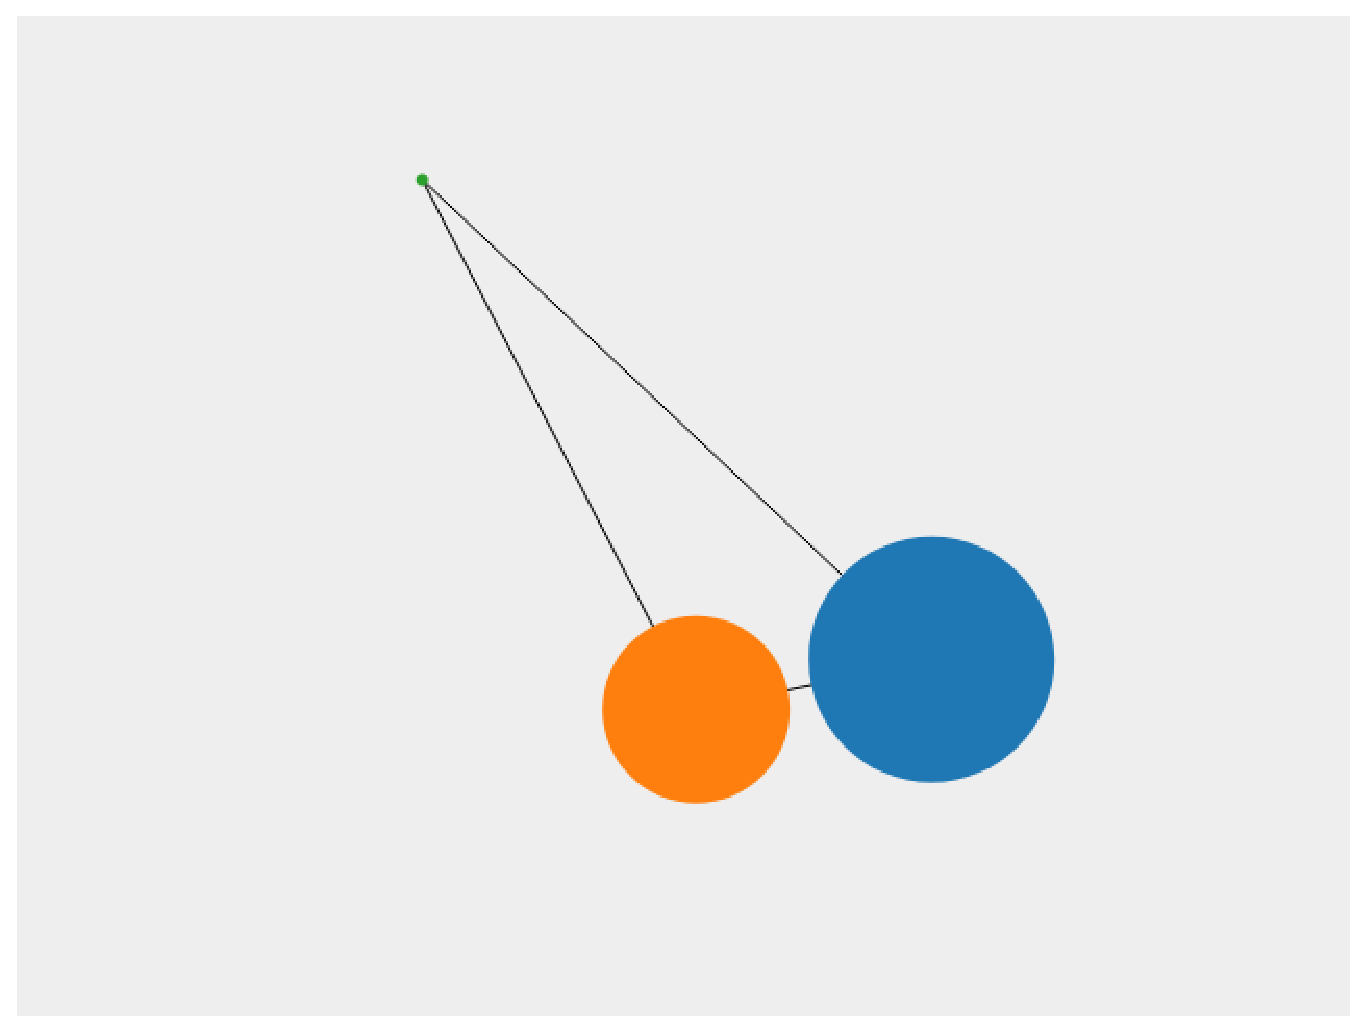
\includegraphics[width=0.5\textwidth]{img/cop-map-graph.eps}
  \caption{本システムによってプロジェクトメンバの関係性を可視化した様子}
  \label{cop-map-graph}
\end{figure}

本システムでは,ノードのレイアウト手法として,力学モデルを採用している.
また,協力してタスクを行った回数によってエッジのバネ定数を変化させることで,
多くのタスクを協力して行ったノードは近くに配置されるようになっている.
これにより,頻繁に協力してタスクを行っているプロジェクトメンバを確認することができる.

また,タスクを行った回数の合計値によってノードの半径を変化させている.
これにより,プロジェクトメンバが正統的周辺参加である可能性を観察することが可能である.
その例として,ノードは小さいが,
他のノードとの繋がりが見られる場合が挙げられる.
この場合は,観察対象となるプロジェクトメンバは,
タスクを行った回数は少ないが,
リソースへのアクセスが可能な状態だと考える事ができる.
本システムによって,
観察される正統的周辺参加の可能性があるプロジェクトメンバを図\ref{cop-map-lpp}に示す.

\begin{figure}[h]
  \centering
  \includegraphics[width=0.5\textwidth]{img/cop-map-lpp.eps}
  \caption{本システムによって観察される正統的周辺参加である可能性のあるプロジェクトメンバ}
  \label{cop-map-lpp}
\end{figure}

さらに,プロジェクトメンバの所属先によってノードの色を変化させることで,
異なる実践共同体に所属するプロジェクトメンバが,
協働でタスクを行っている様子を観察するが可能である.
これにより,異なる色のノードがエッジでつながっている様子から,
布置を観察することができる.
本システムによって観察される布置の例を,
図 \ref{cop-map-overlap}に示す.
このように,布置を観察することで,
異分野横断的なアプリ開発において,
異なる実践共同体が協働的な関係構築を行えているかを確認し,
必要に応じて協働的な関係構築を促すことが可能である.

\begin{figure}[h]
  \centering
  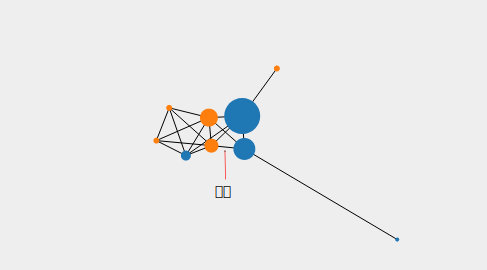
\includegraphics[width=0.5\textwidth]{img/cop-map-overlap.eps}
  \caption{本システムによって可視化された布置}
  \label{cop-map-overlap}
\end{figure}

本システムでは以上のネットワーク構造を,
プロジェクトの時系列順にアニメーションで表示することができる.
これにより,プロジェクトメンバの関係性の変化を観察することが可能である.
ノードの動きから,進行状況によって変化していく,
プロジェクトメンバの軌跡を観察することができる.
これにより,プロジェクトを振り返った際に,
正統的周辺参加であったメンバが中心に移動する様子や,
異なる実践共同体間で布置が構築されていく様子を観察することができる.
% 「布置が構築される」構築されるでいいの?
% 本システムによって観察されるプロジェクトメンバの軌跡を,
% 図\ref{cop-map-trajectory}に示す.

% TODO: 複数の画像をつなげる
% \begin{figure}[h]
%   \centering
%   \includegraphics[width=0.5\textwidth]{img/cop-map-trajectory.eps}
%   \caption{本システムによって観察されるプロジェクトメンバの軌跡}
%   \label{cop-map-trajectory}
% \end{figure}

また,本システムではインタラクティブにデータを観察することが可能である.
本システムで可能なインタラクションは,
ノードのドラッグアンドドロップと,ノードへのマウスオーバーである.
ノードをドラッグアンドドロップすることによって,
ネットワークのレイアウトを調整することが可能である.
また,メンバの詳細情報を確認する際には,
ノードにマウスオーバーすることで,
そのノードに対応するユーザ名を確認することが可能である.
これらのインタラクションにより,
より詳細にプロジェクトメンバの関係性を観察することが可能である.
% インタラクションによって詳細情報を表示している様子を,
% 図\ref{cop-map-detail}に示す.

% TODO: 複数の画像をつなげる
% \begin{figure}[h]
%   \centering
%   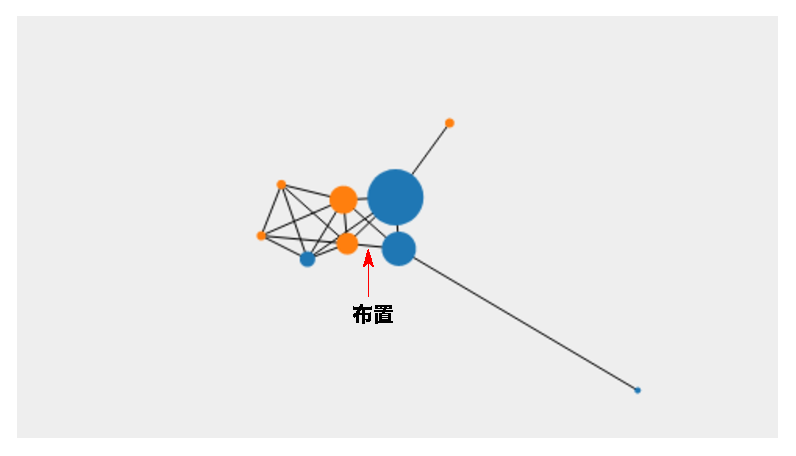
\includegraphics[width=0.5\textwidth]{img/cop-map-detail.eps}
%   \caption{インタラクションによって詳細情報を表示している様子}
%   \label{cop-map-detail}
% \end{figure}


%4
\section{おわりに}
\label{conclusion}
% おわりに

本研究で開発したシステムは,
2021年度9月より実施される学部横断型PBLのアプリ開発を
行う際に使用される予定である.
開発したシステムから,メンバの背景と行為やメンバ間の交渉に着目し,
アプリの機能やUIがどのように決定されていくか分析する予定である.
加えてアプリ開発支援ソフトウェアがアプリ開発の過程にどのように影響を及ぼすかまで含めて分析を行う.

また,本研究において開発した可視化システムについて,
ノードの数が増えた際の可視性の改善が必要だと考えられる.
改善方法については,
論文の共著関係やSNSを対象としたネットワーク可視化の先行研究をもとに検討する予定である.

今後の展望として,
目標とするメンバの関係性のあり方に合わせて,
システムからプロジェクトメンバへの協同作業の提案を行うことも考えられる.
これにより,リソースへのアクセスができていないメンバを正統的周辺参加の状態にするきっかけを作ることができると考えられる.


% \newpage
% \clearpage
% \cleardoublepage

% \\
% \\
% \\
% \\
% \\
% \\
% \\
% \\
% \\
% \\

% FIXME: ここで未来ビジョンを調整する?
\vspace{0mm}

% \section*{謝辞}
% TODO: 書く
% この研究を進めるにあたり,
% 授業内でのデータ収集に協力してくださった学生方.
% データ収集作業を協力してくださった,
% 明星大学情報学研究科情報学専攻の菊池康太さん.
% 田中先生,川俣先生書く?
% シングルブラインド査読のため,謝辞は入れた状態で投稿する.
% 謝辞の例:本研究はJSPS科研費 JP12345678の助成を受けたものです.


% %
% %	参考文献
% %
% \begin{thebibliography}{1}
% \end{thebibliography}

\balance %最後の高さを揃えるために必要 (2012/9/27:watanabe, Igarashi)
\bibliographystyle{jwiss}
\bibliography{sample}

%%%%%%%%%%%%%%%%%%%%%%%%%%%%%%%%%%%%%%%%%%%%%%%%%%%%%%%%%%%%%%%%%%%%%
%%%%%%%%%%%%%%%%%%%%%%%%%%%%%%%%%%%%%%%%%%%%%%%%%%%%%%%%%%%%%%%%%%%%%
%% WISS2012では,「未来ビジョン」は以下のように,本文と同様の2段組形式で記載する.
%% 図を用いても良いが,枠のサイズ(縦93mm)を変更してはならない.
%% (WISS2010では,縦118mmでしたのでご注意下さい)

% \begin{figure*}[!b]
% \setlength{\unitlength}{1mm}\fboxrule=0.5pt

% \vspace{-93mm} %% 未来ビジョンの枠が下がってしまうのを防ぐ WIS2012 カメラレディテンプレで追加  (2012/9/27:watanabe, Igarashi)

% % 未来ビジョンの枠の描画
% \begin{center}
% \framebox[0.95\textwidth]{
% \begin{minipage}{0mm}\begin{picture}(0,91)(0,0)\end{picture}\end{minipage}
% }
% \end{center}
% \vspace*{-93mm}	% 未来ビジョンの枠の縦幅分だけ戻す

% % 未来ビジョンの内容
% \newbox\FUTURE
% \setbox\FUTURE=\vbox{
% \begin{minipage}[b]{0.9\textwidth}
% \begin{multicols}{2}	% 二段組にする
% \section*{未来ビジョン}
% \setlength{\parindent}{10pt}	% 段落先頭の字下げ

% % % % % % % % % % % % % % % % % % % % % % % % % % % % % % %
% %	   未来ビジョンは,下記に記入して下さい		  %
% % % % % % % % % % % % % % % % % % % % % % % % % % % % % % %

% \vspace*{-1mm}

% % フォントサイズ指定
% \normalsize
% %\large
% %\small\setlength{\baselineskip}{12pt}
% %\footnotesize\setlength{\baselineskip}{12pt}

% 本研究のシステムは実証データが未取得なため,
% アプリケーションのデザインを支援するシステムだけでなく,
% アプリケーション開発のプロジェクトにおける
% マネジメントの支援を行うシステムとしても
% 執筆している.
% しかし著者らがこの研究の先に見ていることは,
% 作成される人工物のデザインに関する認識論を変えることである.
% 質の高いプロダクトを作るに当たり,
% 作り手には高い専門性や先端的な技術に焦点が当てられ,
% 多様なメンバ間のコミュニケーションに関しては,
% ものづくりに直接影響を与えるものというより,
% むしろ二次的なマネジメントの視点で語られることが多いのではないだろうか.
% つまり,専門性をもつ人材がそれぞれの立場から分業的に参加し
% アイデア出しやリスク管理,計画を滞りなく進めるためのものという認識である.

% \newpage

% しかし,人の手によって作成される人工物は,
% 各々の専門性に従い,分業的に
% 個々のインプットとアウトプットを正確に行えば
% 生み出されるという単純なものではない.
% むしろ様々な背景を持つメンバ間の交渉や学習,ディスコースの変化といった
% 人間関係のあり方それ自体が人工物の
% デザインにも大きく影響する.人工物の生成過程については
% 状況論的な観点から過去研究でも示されている.

% そのため,筆者らは人工物としてのソフトウェア開発においても,
% メンバ間の関係構築のあり方そのものからデザインを考える認識論を持って
% アプリケーションを作成する必要があると考えている.
% 本研究で開発したシステムがその手助けに
% なるように今後の研究を進めて行きたい.

% .
% %% 文章を補う図表を利用してもよい.
% \vspace*{5mm}
% \includegraphics[width=0.95\columnwidth]{vision.eps}
% % % % % % % % % % % % % % % % % % % % % % % % % % % % % % %
% %	   未来ビジョンは,上記に記入して下さい		  %
% % % % % % % % % % % % % % % % % % % % % % % % % % % % % % %

% \end{multicols}
% \end{minipage}
% }

% % 未来ビジョンの内容の描画
% \newlength{\FUTUREHT}
% \setlength{\FUTUREHT}{\the\ht\FUTURE}	% 未来ビジョンの内容の縦幅保存
% %\typeout{\the\wd\FUTURE}
% %\typeout{\the\ht\FUTURE}
% \hspace*{0.045\textwidth}	% 未来ビジョンの内容の横位置調整
% \box\FUTURE
% %\typeout{\the\FUTUREHT}
% \vspace*{-\the\FUTUREHT}	% 未来ビジョンの内容の縦幅分だけ戻す
% \vspace*{-10.9mm}		% 微調整

% % 未来ビジョンの枠の領域の再確保(これがないと枠が下に沈み込む)
% \begin{center}
% \fboxrule=0pt
% %\fboxrule=2pt	% デバッグ用: コメントアウトをやめて,同じ位置に枠が出るか?
% \framebox[0.9\textwidth]{
% \begin{minipage}{0mm}\begin{picture}(0,91)(0,0)\end{picture}\end{minipage}
% }
% \end{center}
% \end{figure*}

%%%%%%%%%%%%%%%%%%%%%%%%%%%%%%%%%%%%%%%%%%%%%%%%%%%%%%%%%%%%%%%%%%%%%
%%%%%%%%%%%%%%%%%%%%%%%%%%%%%%%%%%%%%%%%%%%%%%%%%%%%%%%%%%%%%%%%%%%%%
\end{document}
